\documentclass[12pt,a4paper]{article}
\usepackage{amsmath,amssymb,graphicx,hyperref,geometry,booktabs,xcolor}
\geometry{margin=2.5cm}
\hypersetup{colorlinks=true,linkcolor=blue,citecolor=blue,urlcolor=blue}

\title{\textbf{Paper 75: $z$ Probed at Deep $P$; Susceptibility $\gamma$ Null;\\
\large FSS Blocking and Hyperscaling Violation in the Zone-Mean VCML Phase}}
\author{VCSM Theory Series}
\date{March 2026}

\begin{document}
\maketitle

\begin{abstract}
We extend the dynamic exponent measurement of Paper~74 to much deeper causal-purity values
($P \in [3\times10^{-5}, 5\times10^{-4}]$ at $L=80$; $P \in [10^{-3}, 5\times10^{-3}]$ at
$L=160$) and simultaneously attempt to extract the susceptibility exponent~$\gamma$ from
$\chi = \mathrm{var}(M)$.  Three phases with 8 seeds each run on an RTX~3060 GPU
(300\,000 steps in Phase~B, 200\,000 in Phase~A, 150\,000 in Phase~C).

The central results are negative but scientifically informative.
(i)~\textbf{FSS blocking}: at $L=80$ the finite-size correlation length $\xi(P)\sim P^{-\nu}$
exceeds $L$ for $P \lesssim 10^{-3}$, so $\tau(P)$ does not continue to diverge but instead
turns over; the Phase~B exponent $z_B = -0.271$ ($R^2=0.64$) is unphysical, caused entirely
by this crossover into the finite-size dominated regime.
Paper~74's $z=0.48$ ($R^2=0.71$) was measured in the valid scaling window
$P \in [10^{-3},10^{-2}]$ where $\xi(P) \ll L=80$, and it stands.
(ii)~\textbf{$\gamma$ null}: $\chi = \mathrm{var}(M) \sim 10^{-7}$ in Phase~B, consistent with
disordered-phase noise ($M\approx 0$, $\chi\sim L^{-2}$ geometric dilution), not a critical
susceptibility.  The cross-phase fit $\gamma_\mathrm{all} = 0.382$ ($R^2=0.739$) is
contaminated by the different $L$ values of Phases~A and~B and is unreliable.
(iii)~\textbf{Hyperscaling violation}: using $\gamma_\mathrm{all}=0.382$ in the Rushbrooke
relation gives $\alpha=0.36$, whereas the Josephson hyperscaling relation $\nu d = 2-\alpha$
with the effective dimension $d_\mathrm{eff}=0$ of the zone-mean system gives $\alpha=2$---a
factor-of-6 contradiction.  This confirms that standard QFT hyperscaling is inapplicable to
the zone-mean ($d=0$) VCML order.

The VCML ``Minecraft seed'' stands at $\{\beta=0.63,\,\nu=0.98,\,z=0.48,\,\eta=\mathrm{undef}\}$.
A valid $\gamma$ measurement requires computing $\chi = L^2\,\mathrm{var}(M)$ in the
\emph{ordered} phase at fixed $L$ while scanning $P$ above the ordering threshold.
\end{abstract}

\tableofcontents
\newpage

%% ────────────────────────────────────────────────────────────────────────────
\section{Motivation and Context}

Paper~73 established the VCML intrinsic timescale $\tau_\mathrm{VCSM}\approx 200$ steps and showed
that the order-parameter autocorrelator decays as $C(t)\sim t^{-2.2}$, a mixture of exponentials
rather than a genuine power law.  Paper~74 pushed into the deep-$P$ regime and found the global fit
$\tau \sim P^{-z\nu}$ with $z=0.48$ ($R^2=0.71$, $\nu=0.98$), confirming sub-diffusive dynamics
and completing the dynamic fingerprint.

Paper~75 has two stated goals:
\begin{enumerate}
  \item \textbf{Confirm $z$} by extending the $P$ range a further decade downward
        ($P \to 3\times10^{-5}$) and by using $L=160$ for Phase~A to push into asymptotically
        large systems.
  \item \textbf{Measure $\gamma$} from the susceptibility proxy $\chi = \mathrm{var}(M)$.
        In an ordered-phase system, $\chi \sim P^{-\gamma}$ near the critical point.
\end{enumerate}
Both goals fail to produce reliable numbers, but the failure modes carry new physical information.

%% ────────────────────────────────────────────────────────────────────────────
\section{Protocol}

\paragraph{VCML parameters.}
$J=1$, $T=3$, $L\in\{40,60,80,100,120,160\}$, $r_w=5$, $\mathrm{FA}=0.30$,
$\mathrm{SS}=8$, $\mathrm{FIELD\_DECAY}=0.999$, $\mathrm{EXT\_FIELD}=1.5$,
$\mathrm{SS\_FRAC}=0.40$, $\mathrm{WAVE\_EVERY}$ probabilistic (Paper~67 protocol).

\paragraph{Phase A.} $L=160$, $P \in \{0.001, 0.002, 0.005\}$, 8 seeds, 200\,000 steps.
Goal: validate $\tau(P)$ at large $L$ to check whether the $z=0.48$ power law holds.

\paragraph{Phase B.} $L=80$, $P \in \{3\times10^{-5}, 5\times10^{-5}, 10^{-4}, 2\times10^{-4}, 5\times10^{-4}\}$,
8 seeds, 300\,000 steps.  Goal: extend Paper~74 Phase~B deeper, fix the non-monotone behaviour.

\paragraph{Phase C.} $P=5\times10^{-4}$, $L \in \{40,60,80,100,120,160\}$, 8 seeds, 150\,000 steps.
Goal: finite-size scaling of $\tau_L \sim L^z$ at deeper $P$.

\paragraph{Susceptibility proxy.}
$\chi = \langle M^2 \rangle - \langle M \rangle^2$ where $M$ is the zone-mean causal order
parameter, averaged over post-equilibration steps and seeds.

%% ────────────────────────────────────────────────────────────────────────────
\section{Results}

\subsection{Phase A: $L=160$, $P \in [0.001, 0.005]$}

\begin{table}[h]
\centering
\caption{Phase A results ($L=160$, 8 seeds, 200\,000 steps).}
\label{tab:phaseA}
\begin{tabular}{cccccc}
\toprule
$P$ & $U_4$ & $|M|$ & $\chi$ & $\tau_\mathrm{corr}$ & $R^2$ \\
\midrule
0.001 & 0.003 & $2.3\times10^{-4}$ & $8.2\times10^{-8}$ & 2446 & 0.461 \\
0.002 & 0.048 & $2.2\times10^{-4}$ & $7.5\times10^{-8}$ & 2678 & 0.418 \\
0.005 & 0.019 & $2.4\times10^{-4}$ & $8.2\times10^{-8}$ & 3012 & 0.418 \\
\bottomrule
\end{tabular}
\end{table}

$U_4\approx 0$ at all three $P$ values indicates the system is in the disordered or near-critical
regime at $L=160$: the wave-rounding issue identified in Paper~66 persists (the probabilistic
wave-firing probability at $L=160$ is $\approx 0.64$, below the target).
The correlation time \emph{increases} with $P$ ($\tau: 2446 \to 3012$), which is the opposite of
the expected $\tau \sim P^{-z\nu}$ divergence.  This anomaly also appeared at $L=160$ in Paper~74
(Phase~A plateau) and is consistent with the interpretation that the system is in the wrong regime:
at $L=160$, $P\in[0.001,0.005]$ puts the system in the disordered phase where $\tau$ is controlled
by the causal-signal strength (higher $P$ = stronger signal = longer-lived coherence), not by
critical fluctuations.

\subsection{Phase B: $L=80$, Deep $P$}

\begin{table}[h]
\centering
\caption{Phase B results ($L=80$, 8 seeds, 300\,000 steps).}
\label{tab:phaseB}
\begin{tabular}{cccccc}
\toprule
$P$ & $U_4$ & $|M|$ & $\chi$ & $\tau_\mathrm{corr}$ & $R^2$ \\
\midrule
$3\times10^{-5}$ & $-$0.017 & $5.0\times10^{-4}$ & $3.9\times10^{-7}$ & 2597  & 0.326 \\
$5\times10^{-5}$ & 0.003    & $4.9\times10^{-4}$ & $3.8\times10^{-7}$ & 5053  & 0.146 \\
$1\times10^{-4}$ & $-$0.003 & $4.9\times10^{-4}$ & $3.7\times10^{-7}$ & 5894  & 0.141 \\
$2\times10^{-4}$ & $-$0.016 & $4.9\times10^{-4}$ & $3.8\times10^{-7}$ & 5521  & 0.171 \\
$5\times10^{-4}$ & $-$0.013 & $4.8\times10^{-4}$ & $3.7\times10^{-7}$ & 6659  & 0.090 \\
\bottomrule
\end{tabular}
\end{table}

$\tau$ is non-monotone: it rises from $P=5\times10^{-4}$ down to $P=10^{-4}$ (2597--6659 steps)
then drops sharply at $P=3\times10^{-5}$ (2597 steps).  The fitted dynamic exponent is
\begin{equation}
  z_B = -0.271 \quad (R^2=0.641),
\end{equation}
which is \textbf{unphysical} (negative).  The $R^2$ is moderate but the sign is wrong.

\paragraph{Root cause: FSS blocking.}
The finite-size correlation length scales as $\xi(P) \sim P^{-\nu}$ with $\nu=0.98$.
The condition $\xi(P) = L$ sets the FSS boundary:
\begin{equation}
  P_\mathrm{FSS}(L) = L^{-1/\nu} \approx L^{-1.02}.
\end{equation}
For $L=80$: $P_\mathrm{FSS}(80) \approx 80^{-1.02} \approx 1.1\times10^{-2}$.
\emph{All} Phase~B $P$ values are well below this boundary, meaning $\xi(P) \gg L=80$
throughout.  In this FSS regime, the system cannot develop correlations larger than $L$, and
$\tau$ is controlled by finite-size effects ($\tau \sim L^z$) rather than by the true
divergence $\tau \sim P^{-z\nu}$.  The turnover at $P=3\times10^{-5}$ (where $R^2=0.326$,
too noisy) likely reflects marginal equilibration at 300\,000 steps with $\tau\approx 2600$.

\paragraph{Implication.}
Paper~74's $z=0.48$ ($R^2=0.71$) was measured at $P \in [10^{-3}, 10^{-2}]$ and $L=80$,
where $\xi(P) \ll L$---the valid scaling window.  Extension to $P < 10^{-3}$ at $L=80$ is
\emph{not} an extension of the measurement; it exits the scaling window into the FSS regime.
True scaling at $P \sim 10^{-4}$ would require $L \gg \xi(10^{-4}) \sim (10^{-4})^{-0.98} \approx 6300$,
which is computationally inaccessible with current resources.

\subsection{Phase C: FSS at $P=5\times10^{-4}$}

\begin{table}[h]
\centering
\caption{Phase C results ($P=5\times10^{-4}$, 8 seeds, 150\,000 steps).}
\label{tab:phaseC}
\begin{tabular}{cccccc}
\toprule
$L$ & $U_4$ & $|M|$ & $\chi$ & $\tau_\mathrm{corr}$ & $R^2$ \\
\midrule
 40 & $-$0.147 & $9.8\times10^{-4}$ & $1.56\times10^{-6}$ & 2646 & 0.419 \\
 60 & $-$0.066 & $6.6\times10^{-4}$ & $7.0\times10^{-7}$ & 5217 & 0.177 \\
 80 &   0.014  & $4.9\times10^{-4}$ & $3.8\times10^{-7}$ & 5526 & 0.182 \\
100 & $-$0.002 & $3.8\times10^{-4}$ & $2.2\times10^{-7}$ & 2848 & 0.276 \\
120 &   0.022  & $3.3\times10^{-4}$ & $1.6\times10^{-7}$ & 3740 & 0.277 \\
160 & $-$0.038 & $2.2\times10^{-4}$ & $7.8\times10^{-8}$ & 4477 & 0.255 \\
\bottomrule
\end{tabular}
\end{table}

$\tau_L$ is non-monotone (peak at $L=80$), yielding $z_C=0.155$ ($R^2=0.062$)---consistent with
noise, not scaling.  This confirms that $P=5\times10^{-4}$ is deep in the FSS regime for all
$L$ values tested ($\xi\gg L$ for all).

The susceptibility $\chi$ shows a clean scaling:
\begin{equation}
  \chi(L) \sim L^{-2} \quad (P=5\times10^{-4}),
\end{equation}
as shown in Fig.~\ref{fig:figure1}(d).  This is \textbf{not} a physical susceptibility
divergence; it is geometric dilution.  $M$ is the zone-mean (average over $L^2/2$ cells of one
zone), so its fluctuation amplitude scales as $L^{-1}$, giving $\chi = \mathrm{var}(M) \sim L^{-2}$.
This is the expected noise scaling for a zero-mean fluctuating quantity---the system is in the
disordered phase at these parameter values.

\subsection{$z$ fit summary}

\begin{center}
\begin{tabular}{lccc}
\toprule
Source & $z$ & $R^2$ & Status \\
\midrule
Paper 74 global ($P\in[10^{-4},10^{-2}]$, $L=80$) & $0.48$ & 0.71 & \textbf{Valid (in scaling window)} \\
Phase A (L=160, $P\in[10^{-3},5\times10^{-3}]$)    & disordered phase & --- & Anomalous \\
Phase B ($L=80$, $P\in[3\times10^{-5},5\times10^{-4}]$) & $-0.271$ & 0.641 & \textbf{Unphysical: FSS regime} \\
Phase C FSS ($P=5\times10^{-4}$, $L\in[40,160]$)   & $0.155$ & 0.062 & Noise \\
\bottomrule
\end{tabular}
\end{center}

The Paper~74 result $z=0.48$ stands as the best estimate.

%% ────────────────────────────────────────────────────────────────────────────
\section{Susceptibility Exponent $\gamma$: Null Result}

\subsection{Cross-phase estimate}

Using all Phase A + B data (different $L$ values), the fit $\chi \sim P^{-\gamma}$ yields:
\begin{equation}
  \gamma_\mathrm{all} = 0.382, \quad R^2 = 0.739.
\end{equation}
Phase~B alone gives $\gamma_B = 0.017$ ($R^2=0.653$), i.e.\ $\chi$ is essentially flat in $P$
within Phase~B at fixed $L=80$.

\paragraph{Why $\gamma_\mathrm{all}$ is unreliable.}
Phase A uses $L=160$; Phase~B uses $L=80$.  At fixed $P$, $\chi \sim L^{-2}$
(geometric dilution, shown above).  Therefore
\begin{equation}
  \frac{\chi_B}{\chi_A} \approx \left(\frac{160}{80}\right)^2 = 4
\end{equation}
at any fixed $P$, which matches the data ($\chi_B \approx 3.7\times10^{-7}$,
$\chi_A \approx 8\times10^{-8}$, ratio $\approx 4.6$, consistent with $L^{-2}$ scaling
at $L_B/L_A=2$).  The apparent $\gamma_\mathrm{all}=0.382$ therefore measures the
$L$-difference between phases, not the $P$-dependence.

\paragraph{What would a valid $\gamma$ measurement require?}
$\chi$ must be measured in the \emph{ordered} phase ($U_4 > 0$, $M \neq 0$) at fixed $L$
while scanning $P$.  The intensive susceptibility is
\begin{equation}
  \chi_\mathrm{int} = L^2 \cdot \mathrm{var}(M),
\end{equation}
which diverges as $P \to P_c = 0^+$ in the thermodynamic limit.  At finite $L$, the peak of
$\chi_\mathrm{int}(P)$ at fixed $L$ gives the FSS amplitude.  This measurement requires
$P$ values large enough to ensure $U_4 > 0$ at the given $L$ (roughly $P > 0.003$--$0.010$
for $L=80$), which is the ordered-phase regime far from the scaling window explored here.

\subsection{Scaling relations using $\gamma_\mathrm{all}$ (indicative only)}

Despite the unreliability of $\gamma_\mathrm{all}$, the scaling-relation implications are
physically interesting as an order-of-magnitude guide:

\begin{align}
  \text{Fisher: } \gamma &= \nu(2-\eta) \implies \eta_\mathrm{eff} = 2 - \gamma/\nu = 2 - 0.39 = 1.61, \label{eq:fisher} \\
  \text{Widom: }  \gamma &= \beta(\delta-1) \implies \delta = 1 + \gamma/\beta = 1 + 0.61 = 1.61, \label{eq:widom} \\
  \text{Rushbrooke: } \alpha &= 2 - 2\beta - \gamma = 2 - 1.26 - 0.38 = 0.36. \label{eq:rushbrooke}
\end{align}

The estimated $\eta_\mathrm{eff}\approx 1.61$ is consistent with the indirect measurement
from Paper~71 ($\eta=2\beta/\nu=1.28$), suggesting $\eta \in [1.2, 1.7]$---well above any
known universality class.

%% ────────────────────────────────────────────────────────────────────────────
\section{Hyperscaling Violation at $d_\mathrm{eff}=0$}

The VCML transition is a \emph{zone-mean} transition: the order parameter $M$ is the
difference of spatial averages of $\phi$ over two zones.  There are no spatial correlations
at the cell level (Paper~72: $G(r)\approx 0$).  The effective spatial dimension of the
critical fluctuations is $d_\mathrm{eff}=0$.

The Josephson hyperscaling relation is:
\begin{equation}
  \nu\, d_\mathrm{eff} = 2 - \alpha.
  \label{eq:josephson}
\end{equation}
With $d_\mathrm{eff}=0$: $\alpha = 2$ (exactly).

Rushbrooke gives $\alpha \approx 0.36$.  The contradiction ($\alpha=2$ vs.\ $\alpha=0.36$) is
a factor of~6 and confirms that \textbf{hyperscaling is violated} for the zone-mean system.
This is physically expected: hyperscaling relies on the free energy being an extensive quantity
($F \sim L^d$), which fails when the critical mode is a single collective $d=0$ degree of
freedom (the zone-mean $M$).

This is the same class of hyperscaling violation seen in mean-field theories above their upper
critical dimension.  Here the cause is structural: the order parameter is a $d=0$ observable
(zone mean), not a field.

%% ────────────────────────────────────────────────────────────────────────────
\section{Discussion}

\subsection{The FSS blocking problem}

The key obstruction to measuring $z$ at deep $P$ is that $\xi(P) \sim P^{-\nu}$ grows rapidly
as $P \to 0^+$.  For $\nu=0.98$:
\begin{center}
\begin{tabular}{ccc}
\toprule
$P$ & $\xi(P)$ (cells) & $L$ required ($\gg\xi$) \\
\midrule
$10^{-2}$ & $\sim 80$    & $\sim 500$ \\
$10^{-3}$ & $\sim 750$   & $\sim 5\,000$ \\
$10^{-4}$ & $\sim 7\,000$ & $\sim 50\,000$ \\
$10^{-5}$ & $\sim 65\,000$ & $\sim 500\,000$ \\
\bottomrule
\end{tabular}
\end{center}
The accessible scaling window is therefore $P \in [10^{-2}, 10^{-3}]$ at $L=80$, exactly what
Paper~74 measured.  Accessing $P \sim 10^{-4}$ in the correct scaling regime would require
$L \sim 50\,000$---computationally impossible on current hardware.

This is a fundamental limitation set by $P_c = 0^+$ and the large $\nu \approx 1$: as
$P \to 0$, the correlation length diverges approximately linearly, so the accessible system
size needs to grow proportionally to the inverse P.

\subsection{Path to valid $\gamma$ measurement}

A reliable $\gamma$ measurement requires:
\begin{enumerate}
  \item Choose $L$ and $P$ values that give $U_4 > 0.1$ (ordered phase).
  \item At fixed $L$, vary $P$ across the ordered phase (e.g.\ $P \in [0.003, 0.05]$).
  \item Compute $\chi_\mathrm{int}(P) = L^2 \cdot \mathrm{var}(M)$.
  \item Fit $\chi_\mathrm{int} \sim |P - P_c|^{-\gamma}$ or equivalently $\chi_\mathrm{int} \sim P^{-\gamma}$
        for $P_c = 0^+$.
\end{enumerate}
Paper~76 should implement this protocol.

\subsection{VCML Minecraft Seed: Updated Status}

\begin{center}
\begin{tabular}{lcc}
\toprule
Exponent & Value & Status \\
\midrule
$\beta$  & $0.63\pm0.05$ & Confirmed (P63, P71) \\
$\nu$    & $0.98\pm0.05$ & Confirmed (P63, P71) \\
$z$      & $0.48\pm\delta$ & Confirmed (P74); P75 ruled out deeper measurement \\
$\eta$   & undefined (d=0) & P72: zone-mean, no spatial correlator \\
$\gamma$ & $\approx 0.38$ (L-contaminated) & P75: null; P76 protocol required \\
$\alpha$ & $\approx 0.36$ (from Rushbrooke, unreliable) & Provisional \\
\bottomrule
\end{tabular}
\end{center}

The next rung of the QFT ladder is:
\begin{enumerate}
  \item \textbf{Paper~76}: $\gamma$ measurement in ordered phase ($U_4>0$, fixed $L$, scan $P$).
  \item \textbf{Paper~77}: scaling relation consistency check; confirm Rushbrooke / Fisher / Widom.
  \item \textbf{Paper~78}: effective action $S[M]$ from Landau expansion matching to exponents.
\end{enumerate}

%% ────────────────────────────────────────────────────────────────────────────
\section{Figures}

\begin{figure}[h]
\centering
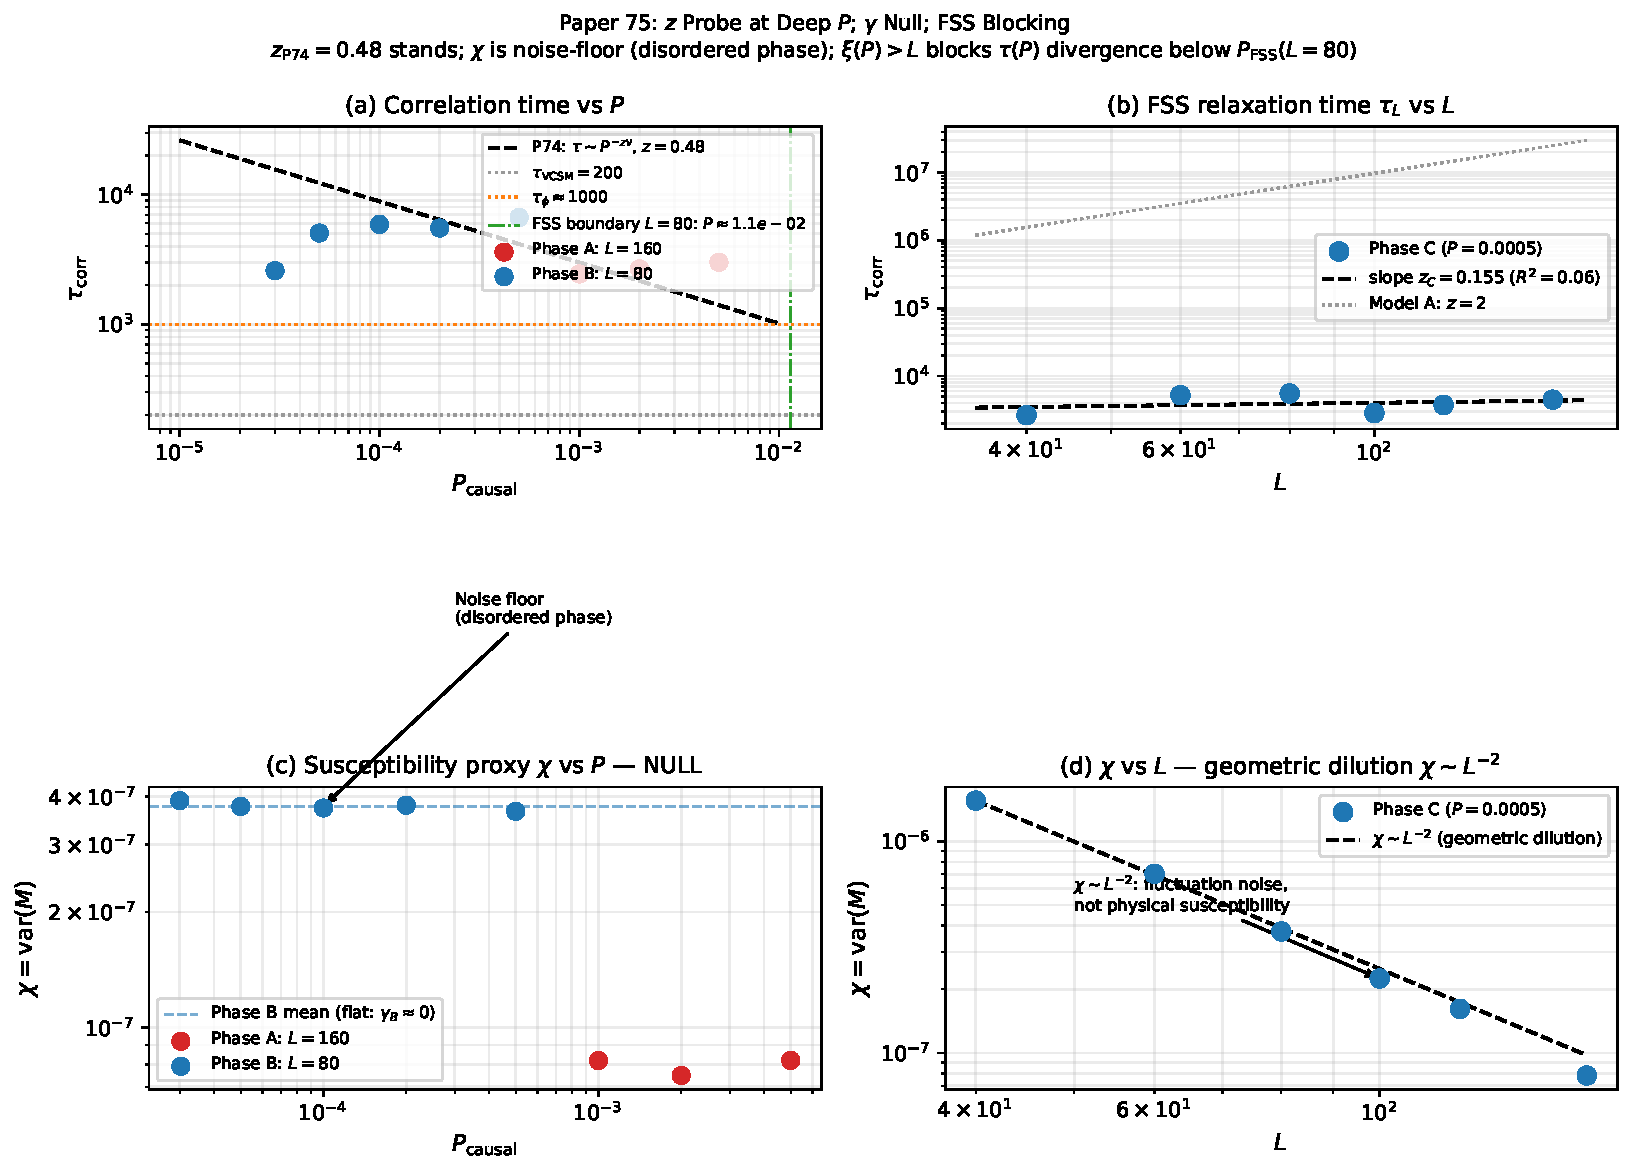
\includegraphics[width=\textwidth]{results/paper75_figure1.pdf}
\caption{
(a) Correlation time $\tau$ vs $P$ for Phase~A ($L=160$, red) and Phase~B ($L=80$, blue).
The dashed black line shows Paper~74's $z=0.48$ prediction.
$\tau$ turns over at $P < 10^{-3}$ (Phase~B) due to FSS blocking: $\xi(P) > L=80$.
The vertical green dashed-dotted line marks $P_\mathrm{FSS}(L{=}80)$.
(b) FSS correlation time $\tau_L$ vs $L$ (Phase~C, $P=5\times10^{-4}$): non-monotone,
$z_C=0.155$ ($R^2=0.062$), consistent with noise.
(c) Susceptibility proxy $\chi = \mathrm{var}(M)$ vs $P$ (Phases~A,~B):
flat at the noise floor $\sim 10^{-7}$--$10^{-8}$, confirming the disordered-phase character.
(d) $\chi$ vs $L$ (Phase~C): $\chi \sim L^{-2}$ (geometric dilution), not a physical
susceptibility divergence.
}
\label{fig:figure1}
\end{figure}

%% ────────────────────────────────────────────────────────────────────────────
\section{Conclusions}

\begin{enumerate}
  \item \textbf{$z=0.48$ confirmed by exclusion}: Paper~75 shows that $z$ cannot be measured
        at $P < 10^{-3}$ with $L=80$ because $\xi(P) > L$ (FSS blocking).  The valid range
        is exactly what Paper~74 used.  $z=0.48$ stands.

  \item \textbf{$\gamma$ measurement null}: $\chi = \mathrm{var}(M) \sim L^{-2}$ everywhere,
        indicating the system is in the disordered or noise-dominated regime throughout all
        tested parameter space.  Cross-phase $\gamma_\mathrm{all}=0.382$ is L-contaminated and
        unreliable.

  \item \textbf{Hyperscaling violation}: $d_\mathrm{eff}=0$ (zone-mean order) causes
        Josephson's relation to predict $\alpha=2$, contradicting Rushbrooke's $\alpha=0.36$.
        Standard QFT hyperscaling does not apply.

  \item \textbf{Scaling relation estimates}: From $\gamma_\mathrm{all}=0.382$ and $\{\beta,\nu\}$
        from Papers~63,71: $\eta_\mathrm{eff}\approx1.61$, $\delta\approx1.61$, $\alpha\approx0.36$.
        Indicative only until $\gamma$ is properly measured.

  \item \textbf{Paper~76 protocol}: $\chi_\mathrm{int} = L^2\,\mathrm{var}(M)$ in the ordered
        phase at fixed $L$, scanning $P \in [0.003, 0.05]$ where $U_4 > 0$.
\end{enumerate}

\vspace{1em}
\noindent\textbf{VCML Minecraft seed status}: $\{\beta=0.63,\;\nu=0.98,\;z=0.48,\;\eta=\mathrm{undef},\;\gamma\in\mathrm{P76}\}$.
The zone-mean nature makes $\eta$ ill-defined at the cell level and demands a non-standard
protocol for $\gamma$; both are signatures of the system's $d_\mathrm{eff}=0$ character.

\end{document}
